Even for the HL-LHC with almost 3\abinv of data, none of the HH analyses can reach the discovery sensitivity, thus the goal for all HH analyses now and in the nearest future is to contribute to the grand combination and only in this collaborative way to achieve the desired sensitivity. From the recent results of the HL-LHC projection analysis ~\cite{CMS-PAS-FTR-18-019}: "the statistical combination of the five decay channels results in an expected significance for the standard model HH signal of 2.6$\sigma$". This is a clear sign that more data are needed. However, many Higgs analysts would agree that new statistical and MVA tools should be developed/employed. Thus, the next iteration of this analysis will most likely use a sophisticated neural network not only for the signal-background separation, but also for lepton reconstruction, etc. 

The present limits computed for the 2016 dataset are far beyond the sensitivity to rule out the WED theory in the consideration. The most recent grand combination results for the spin 0 case ~\cite{CMS-PAS-HIG-17-030} are shown at the Fig. \ref{HH_combo}. As we can see, 

\begin{figure}[H]%hbpt?                                                                       
  \begin{center}
    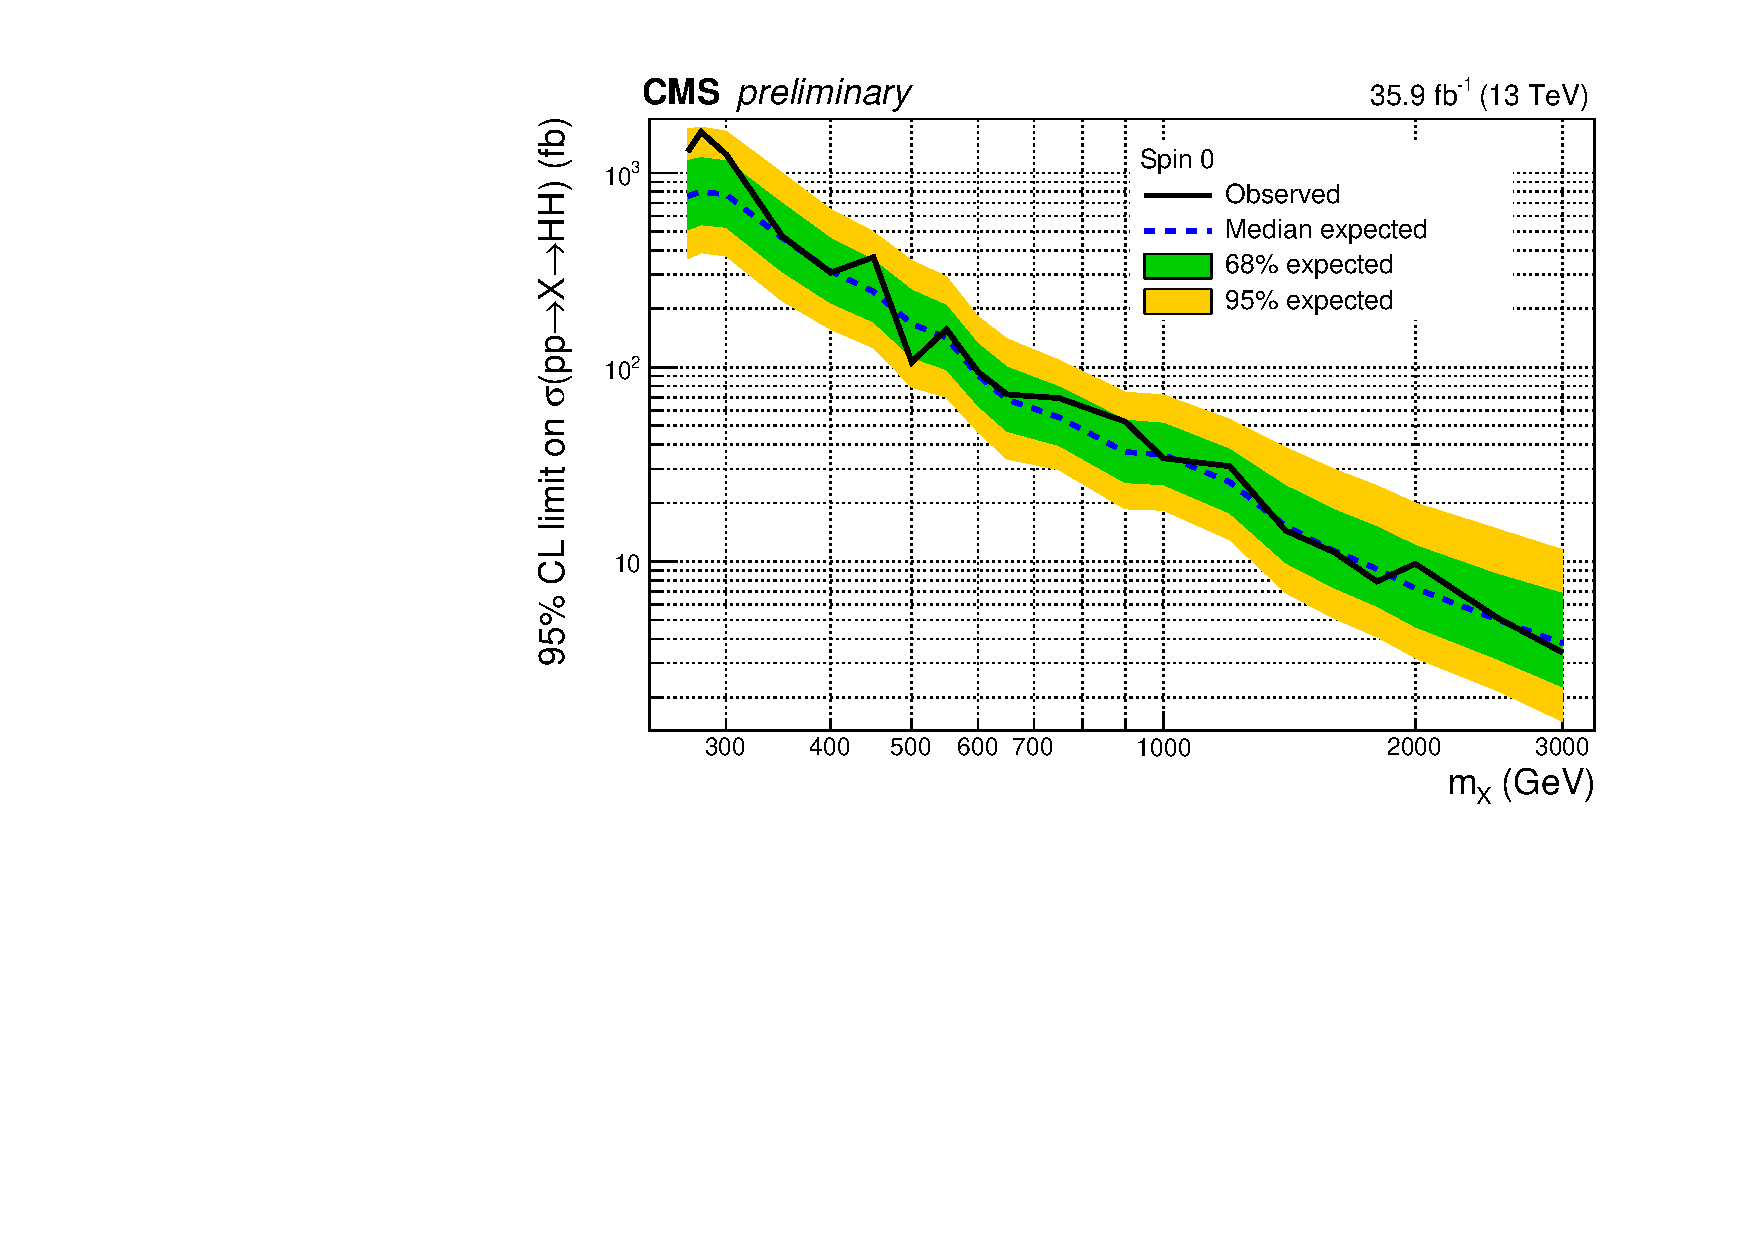
\includegraphics[width=0.85\textwidth]{HH_combo.pdf}
    \caption{ Combination of HH channels for 2016 data. Expected (dashed) and observed (solid line) 95\% CL exclusion limits are shown. The results describe the production cross section of a narrow width spin zero resonance decaying into a pair of SM Higgs bosons.  }
    \label{HH_combo}
  \end{center}
\end{figure}










This analysis note presented the search for the double Higgs boson production mediated by the intermediate graviton (and separately) by the radion in the bbZZ channel with the 2 bjets, 2 leptons, 2 neutrinos final state with the $35.9\fbinv$ 2016 dataset. Limits on the process mediated by the heavy resonance are obtained. Results are shown for the combined data utilizing both the dimuon and the dielectron channels. The mass range covered in the measurement is from 250 GeV to 1000 GeV.

This note presents a search for the production of two Higgs bosons
through narrow resonances, a KK graviton (spin-2) and a radion (spin-0), where one of the Higgs bosons decays to
two \Pqb quarks while the other decays to a pair of \PZ bosons which, in
turn, decay to a pair of neutrinos and a pair of electrons or muons.
The search is performed with the $35.9\fbinv$ of 2016 data set
collected by the CMS experiment at the LHC in proton-proton collisions at
$\sqrt{s} = 13 \TeV$.

No statistically significant deviations from the SM predictions for
background processes have been observed, and 95\% upper confidence limits are reported for production cross section
of a KK graviton/radion times the branching fraction of the subsequent decay into an
HH system. The limits are derived for resonance masses in the 250 GeV to 1 TeV range.
%The limits are set for the mass range of the resonance from 250~GeV to 1~TeV.                                                                                            
%While the computed limits do not lead to exclusion of any resonance mass ranges, when added to other double Higgs decay channels' results from CMS, they will enhance th\
e combined exclusion range.                                                                                                                                               


%The results for the resonant HH production have been presented with                                                                                                      
%the $35.9\fbinv$ of 2016 data set collected from the LHC proton-proton collisions at                                                                                     
%$\sqrt{s} = 13 \TeV$. The results are compatible with the SM within                                                                                                      
%the uncertainties. 95 $\%$ CL upper limits (see Table ~\ref{tab:finalLimits}) are set on the production                                                                  
%of a Higgs boson pair through the intermediate RS KK-graviton in the range of masses from 250 to 1000 GeV.                                                               
%%Interpretation of the model independent results for a narrow spin-2 resonance decaying to a pair of Higgs bosons is done within a WED framework for a graviton particle\
.                                                                                                                                                                         

